\appendix

\sectionlink{Ohmicな振る舞いを示す例}\label{app0}

（$\pi$で記述される）系が調和振動子の「熱浴」と線形に結合する、よく知られた場合を考えよう。そのとき\cite{weiss,calzetta}
\beq
\label{Ltot}
\calL_{\rm tot} =  \calL_\pi(\pi,\dot\pi) + \calL_{\rm int}(q,\pi) + \calL_q(q,\dot q),
\eeq
ただし、
\beq
\calL_\pi = \frac{1}{2} \dot\pi^2 - \frac{1}{2}\omega_0^2 \pi^2,~ \calL_q = \sum_\alpha \frac{1}{2} \dot q_\alpha^2 - \frac{1}{2}\omega_\alpha^2 q_\alpha^2,~\calL_{\rm int} = -c_\alpha \sum_\alpha \pi q_\alpha.
\eeq
このとき運動方程式は
\bea
\ddot\pi +\omega_0^2 \pi + \sum_\alpha c_\alpha q_\alpha &=& 0 \label{eompia}\\
\ddot q_\alpha +\omega_\alpha^2 q_\alpha + c_\alpha\pi &=& 0 \label{eomqa}.
\eea
となる。式(\ref{eomqa})の解を式(\ref{eompia})に代入すると、いわゆるLangevin型の方程式を得る：
\beq
\label{eom2n}
\ddot\pi +\omega_0^2 \pi +  \int dt' \tilde\gamma(t-t')\pi(t') = J(t),
\eeq
ここで、
\beq
J (t)= -\sum_\alpha c_\alpha q^{\pi=0}_\alpha(t),
\eeq
$ q^{\pi=0}_\alpha (t)$は$\pi$が存在しない場合の振動子の古典的軌道を表し、
\beq
\label{gammattp}
\tilde\gamma(t-t') \equiv \sum_\alpha c_\alpha^2 G^\alpha_{\rm ret}(t-t').
\eeq
である。上式では、振動数$\omega_\alpha$の調和振動子の遅延Green関数
\beq
G_{\rm ret}^\alpha(t-t') = \theta(t-t') \frac{\sin(\omega_\alpha(t-t'))}{\omega_\alpha},
\eeq
を導入した。
ここで、環境中の各振動子について独立に選ばれたランダムな初期条件を仮定すると、$J(t)$を確率変数とみなすことができる。
その場合、$\pi$は$J(t)$によって誘起される「雑音」の影響を受けるため、その動力学は確率的な性質を帯びる。
素粒子物理学の言葉でいえば、振動子の熱浴を積分消去し、一般化された摩擦項と雑音を含む$\pi$場の有効運動方程式を得たことになる。（ただし、本論文で強調したように、この運動方程式は$\calL(\pi,\dot\pi)$の形のLagrangianからは導かれない。）\\

このままでは、$\pi$の運動方程式は非局所的である（係数$c_\alpha$にきわめて特殊な性質を仮定する場合を除く\cite{weiss, calzetta}）。それでも、以下で論じるように、定数$\gamma$を用いて
\beq
\label{imgam2}
{\rm Im} \tilde\gamma(\omega) \simeq  \gamma \omega,
\eeq
となる状況があり、このとき運動方程式は望む形
\beq
\label{eom1n}
\ddot\pi + \gamma\dot\pi+ \omega_0^2\pi = J
\eeq
をとる。ここでは$\langle J\rangle =0$であり、繰り込みによる寄与を含むように$\omega_0$を再定義した。\\

式(\ref{Ltot})のようなLagrangianによる記述は、いわゆるRubin模型において対角化の後に現れる。この模型では、重い質量$M$が、質量$m$、ばね定数$m\omega_R^2/4$の調和振動子からなる半無限の鎖に結合している（$\omega_R$は到達可能な最大振動数である）\cite{weiss}。この場合、\cite{weiss}
\beq
\label{imrubin}
{\rm Im} \tilde\gamma_R \simeq \omega~\frac{m \omega_R}{M} \sqrt{1-\omega^2/\omega_R^2}~\theta(\omega_R-\omega),
\eeq
となり、$\omega \ll \omega_R$では$\gamma \sim (m/M)\omega_R$として式(\ref{imgam})の型になる。\footnote{$t \gg \omega_R^{-1}$での漸近的振る舞いは$\gamma_R(t) \sim \frac{m}{M} \sqrt{\frac{\omega_R}{t^3}}\sin\omega_R t$で与えられ、式~(\ref{drude})の場合よりも減衰が緩やかであることに注意されたい。}\\

運動方程式に非局所的効果が現れるのは、環境が対象の系に反作用できるためである。したがって、局所近似を得るためには、系のエネルギーが環境へ散逸し、環境からの反作用の効果が無視できる（あるいは実験の継続時間よりもはるかに長い時間スケールで初めて重要になる）状況を考えればよい。

Rubin模型と同じ考え方に基づく例として、質量$M$の環を半無限の紐に取り付けた場合を考えよう。$x>0$と時間の関数としての紐の高さを$y(x,t)$と表し、環の位置を$\pi(t) \equiv y(0,t)$とすると、運動方程式は
\bea
\frac{\partial^2 y}{\partial x^2} &=& \frac{\partial^2 y}{\partial t^2} \\
M \ddot \pi &=& F \left(\frac{\partial y}{\partial x}\right)_{x=0}
\eea
となる。ここで$F$は紐に働く単位長さ当たりの張力であり、伝播速度を1とする単位系を用いている。波動方程式から
\beq
\left(\frac{\partial y}{\partial x}\right)_{x=0}
= \pm \left(\frac{\partial y}{\partial t}\right)_{x=0},
\eeq
が成り立つ。外向きの波だけを許す境界条件（すなわち$y(x,t) = f(x-t)$）を選ぶと、
\beq
\ddot \pi + \gamma \dot \pi =0,
\eeq
を得る。ただし$\gamma = F/M$である。ここで振動数$\omega_0$のばねを環に取り付けるだけで、$J=0$の場合の式(\ref{eom1n})に戻る。（紐はRubin模型の連続極限に対応することに注意されたい。この極限では$m\omega_R$を有限に保ちながら$m\to 0$、$\omega_R\to\infty$とするので、式(\ref{imrubin})から、すべての時刻にわたって一定の$\gamma_R$が得られる。）

より現実的な設定では、長さを$L$とした紐の一端を固定することを考えられる。このとき、波は$t_B\sim L$程度の時間スケールで反射して戻り、非局所的効果を生じる。このような状況でも、関心のある時間スケールが$t \ll t_B$である限り、局所近似は有効である。

\sectionlink{光学定理}\label{appA}

本論文では散逸を扱っているが、得られた結果は依然としてユニタリ性と整合的である。このつながりをより明確にするために、$\pi$粒子の前方散乱振幅を考えよう。図\ref{fig1}ではこれを「自己エネルギー」図として描いており、波線が$\pi$の伝播関数を表す。

\begin{figure}[h!]
\centering
    \centering
    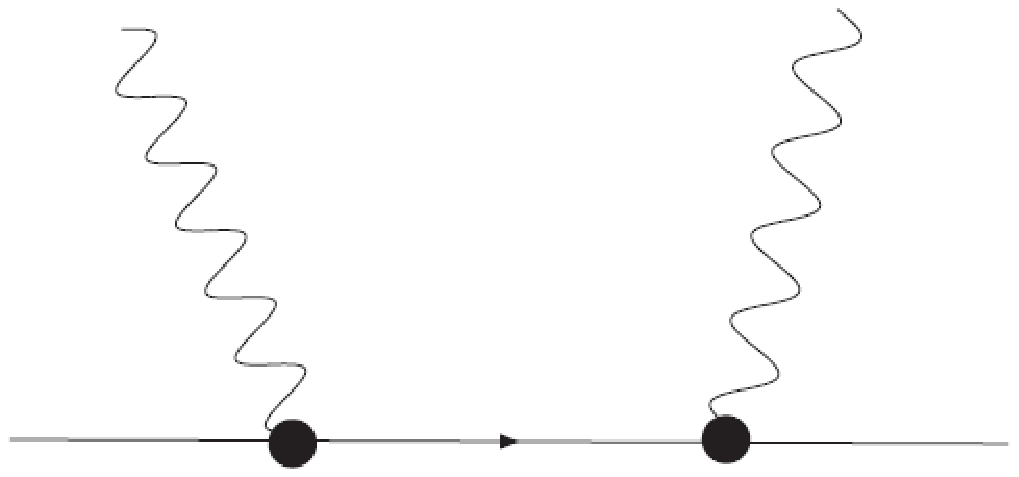
\includegraphics[width=6.5cm]{abs_cropped}
\caption{波線は$\pi$に対応し、黒い相互作用点は$\calo\pi$結合の挿入である。点を結ぶ線は、式(\ref{tfeynm})のFeynmanの時間順序積を表す。}
\label{fig1}
\end{figure}

実際、この振幅は時間順序積
\beq
\label{tfeynm}
\langle T (\delta\calo(x)\delta\calo(y))\rangle,
\eeq
に比例する。これはFeynman伝播関数$iG_{\rm F}(x-y)$とも呼ばれ、$\calL_{\rm int} = \delta\calo \pi.$をもつ通常の経路積分形式で$\delta\calo$を積分消去すると現れる。光学定理という形で表されたユニタリ性は、この振幅の虚部が単位時間当たりの全エネルギー損失と関係しなければならないことを示している\cite{dis1,dis2}。したがって、
\beq
{\rm Im}{\cal A}_{\pi\to\pi} \simeq {\rm Im}\, G_{\rm F}(\omega)
\eeq
および（$\omega>0$に対して）
\beq
\label{imgimf}
{\rm Im}\,G_{\rm F}(\omega) = {\rm Im}\,G_{\rm ret}^\calo(\omega),
\eeq
を用い、（遷移率をエネルギーに換算するため）$\omega$を掛けると、
\beq
\frac{dE}{dt} \simeq \omega{\rm Im}\,{\cal A}_{\pi\to\pi} \simeq \omega{\rm Im}G_{\rm ret}^\calo(\omega).
\eeq
を得る。この式が、$\gamma\dot\pi$という形の散逸項から従う条件
\beq \frac{dE}{dt} = \gamma \dot\pi^2, \label{dedtap}\eeq
に一致することを要求すると、予想どおり（$\omega>0$に対して）
\beq
{\rm Im}G_{\rm ret}^\calo(\omega) \simeq \gamma \omega
 \eeq
と結論される。一般には式(\ref{dedtap})はより複雑になりうるが、この手順は任意の$\omega$の関数に一般化できる\cite{dis1,dis2}。\\

読者は、遅延伝播関数ではなくFeynman伝播関数が現れることに戸惑うかもしれない。しかし、文献\cite{nrgr2,nrgr2p,nrgr2p2,radgo,eftrev}の重力放射の有効場理論（EFT）で行われているのと同様に、Feynman境界条件を用いて自己エネルギー図の虚部を全放射パワー（またはエネルギー損失）と関係づけることができる。重要なのは、$\delta\calo$の「in」状態と「out」状態が真空になるように（例えば外部からの重力放射がないように）境界条件を選ぶと同時に、全放射パワーを正確に表す虚部が生じるという点である。別の見方として、結合$\delta\calo \pi$によって誘起される全遷移率が、次の量に比例することに注目してもよい（議論を簡単にするため${\bf k}$の因子を省略する）：
\be
\sum_N    \langle \pi,0|\pi\delta\calo(t)|0,N\rangle \langle \pi,0| \pi\delta\calo(0)|0,N\rangle^\star = \sum_N  \langle 0|\delta\calo(0)|N\rangle \langle N|\delta\calo(t)|0\rangle = \langle 0| \delta\calo(0)\delta\calo(t)|0\rangle,
\ee
これは、可能なすべての（中間）状態$N$にわたる放出振幅${\cal A}_{\pi \to N}$の絶対値の二乗の和にほかならない。そこで、（$\omega>0$で成立する）関係
\beq
\int dt\, e^{i\omega t} \langle 0| \delta\calo(0)\delta\calo(t)|0\rangle = 2\,{\rm Im}\; i \int dt\, e^{i\omega t} \langle 0| T(\delta\calo(0)\delta\calo(t))|0\rangle,
\eeq
を用いると、（$\omega$を掛けた後で）先ほどの結果を再現する。これは光学定理の働きそのものである。少し微妙なのは、経路積分の方法から式(\ref{dret0})の正しい遅延境界条件をどのように得るかという点である。しかし、いわゆる「in-in」形式ではこれが可能である\cite{calzetta, weiss, Zhang}。（重力放射反作用の場合の議論については\cite{radre}を参照。）

\sectionlink{遅延Green関数} \label{appB}

この付録では遅延Green関数の基本的な性質をいくつか示し、特に、本論文全体を通じて用いた${\rm Im}G^\calo_{\rm ret} \simeq \omega$となる例を議論する。

遅延Green関数の公理的な性質から始め、空間運動量がゼロの場合を考えよう。まず、因果律から、$G_{\rm ret}^\calo(\omega)$は${\rm Im}\, \omega>0$において$\omega$の解析関数である。さらに、その虚部は$\omega$の奇関数である：
\beq
\label{prop2}
{\rm Im}\,G_{\rm ret}^\calo(-\omega)=-
{\rm Im}\,G_{\rm ret}^\calo(\omega).
\eeq
また、実部と虚部はKramers-Kronig関係によって結びついている：
\bea\label{kk}
\text{Re}\,G_{\rm ret}^\calo(\omega) & = & P \int_{-\infty}^\infty \frac{d\omega'}{\pi} \frac{\text{Im}\,G_{\rm ret}^\calo(\omega')}{\omega'-\omega}, \\
\text{Im}\,G_{\rm ret}^\calo(\omega) & = & - P \int_{-\infty}^\infty \frac{d\omega'}{\pi} \frac{\text{Re}\,G_{\rm ret}^\calo(\omega')}{\omega'-\omega},
\eea
ここで$P$は主値を表す。これより
\beq
\label{prop1}
\int_{-\infty}^{+\infty} d\omega' \frac{{\rm Im}\, G_{\rm ret}^\calo(\omega')}{\omega'} < \infty,
\eeq
が従い、さらに
\beq
{\rm Im}\,G_{\rm ret}^\calo(\omega \to 0) \to 0. \label{wtozero}
\eeq
を得る。式(\ref{wtozero})は$\omega=0$に極が存在することを禁じるが、原点から離れた領域で式(\ref{tildG})の振る舞いをすることまでは排除しない。このことは付録\ref{mag00}で示す。\\

次に、電気伝導の例を調べよう。よく知られているように、導体中の電流と電場の関係は
\beq
{\bf j}_e = -i \omega \sigma(\omega) {\bf A}(\omega),
\eeq
で与えられる。ただし${\bf E}(\omega) = -i\omega {\bf A}(\omega)$である。線形応答理論を用いると、次の式（Kubo公式）を示せる：
\beq
{\rm Re}\, \sigma(\omega) = \frac{{\rm Im}\, G^j_{\rm ret}(\omega)}{\omega},
\eeq
ここで$G^j_{\rm ret}$は電流${\bf j}_e$の遅延Green関数である。一般に、このGreen関数は\cite{forster}
\beq
G^j_{\rm ret}(\omega) = \frac{\alpha_j M_j(\omega)}{\omega + M_j(\omega)},
\eeq
とパラメータ表示できる。ここで$M_j(\omega)$は「記憶関数」、$\alpha_j$は定数である。系によっては、ある周波数域で$M_j(\omega) \sim i/\tau_j + O(\omega\tau_j)$と近似できる。$\tau_j$は「記憶時間」であり、この場合
\beq
\label{Gjret}
G^j_{\rm ret}(\omega) \simeq -\frac{\sigma_j}{i\omega-\omega_D} \quad\Rightarrow\quad {\rm Im} G^j_{\rm ret}(\omega) \simeq \frac{\sigma_j\omega}{\omega^2 + \omega_D^2},
\eeq
となる。ただし$\omega_D \simeq 1/\tau_j$、$\sigma_j = \alpha_j \omega_D$である。$\omega \ll \omega_D$では、式(\ref{drude})のDrude模型と同じ振る舞いを得る。

Re $G^j_{\rm ret} \simeq \sigma\omega_D$も成り立つことに注意されたい（これは明らかに式(\ref{kk})の分散関係と整合的である）。これは原理的にはGreen関数の実部に大きな補正が生じることを意味する。${\calo}$演算子がこの形のGreen関数をもつ場合、$\pi$に大きな質量を生じさせる可能性がある。本論文で関心をもつ場合には、近似的なシフト対称性が存在する場合のように、大きな寄与を禁じ、$m_\pi$を$O(\epsilon)$に保つ機構があると仮定した。

\sectionlink{分離極限}\label{appdec}

単一場インフレーションでは、スローロール近似のもとで$\delta N$と$\delta N_i$が抑制されることを示せる。したがって、de Sitterに\textit{近すぎない}模型では、$O(\epsilon)$の効果を除いて$\pi$の理論だけを扱えばよい\cite{eft1}。ここでは、追加自由度（ADOF）を含めても分離が成立することを論じ、混合項の構造について一般的な考察を述べる。この節では、特に断らない限り$M^2_p=1$の単位系を用いる。\\

よく知られているように、背景の全${\bar T}^{\mu\nu}$は完全流体の形
\beq
{\bar T}_{\mu\nu} = (\bar \rho_{tot}+\bar p_{tot}){\bar u}_\mu {\bar u}_\nu + \bar g_{\mu\nu} \bar p_{tot}
\eeq
をとる（これは等方性と一様性の条件から従う）。以下ではNewtonianゲージを用い、
\beq
g_{00} = -1-2\Phi,~ g_{0i}=0,~ g_{ij} = \bar g_{ij} (1-2\Psi).
\eeq
とする。

一次のスカラー摂動に注目すると、
\bea \label{stresslin}
\delta T_{ij} &=& -2\Psi \bar g_{ij} \bar p_{tot}  + \bar g_{ij} \delta p + \delta \tau_{ij}\\
\delta T_{00} &=& 2 \bar \rho_{tot} \Phi + \delta \rho \\
\delta T_{i0} &=&   - (\bar\rho_{tot}+\bar p_{tot}) \partial_i \delta u,
\eea
となる。ここにはADOFによって誘起される散逸項$ \delta \tau_{ij}$を含めた。（ADOFは$\delta\rho, \delta p$にも寄与することを忘れてはならない。）
運動方程式は\cite{weinberg}
\bea
\label{b6}
\partial_j\left(\delta p +2 \partial_0(\epsilon H^2\delta u) + 6\epsilon H^3\delta u + 2\epsilon H^2\Phi\right) +   \partial_i\delta\tau^i_j &=& 0\\
\delta\dot\rho + 3 H(\delta\rho+\delta p) + H\delta \tau^i_i + 2\epsilon H^2 \left(\frac{\nabla^2\delta u}{a^2} -3 \dot \Psi\right) &=& 0\label{b7}\\
\frac{\nabla^2\Psi}{a^2}-\frac{1}{2}\delta \rho + 3 \epsilon H^3 \delta u &=& 0\label{b8}\\
\frac{1}{a^2} \left( \partial_i\partial_j - \frac{1}{3} \delta_{ij} \nabla^2\right) (\Psi-\Phi)&=& \left(\delta\tau^i_j-\frac{1}{3}\delta_{ij} \delta\tau^l_l\right) \label{b9}
\eea
となる。ここでは$\bar \rho_{tot}+\bar p_{tot} = -2\dot H= 2H^2\epsilon$、（$\epsilon = -\dot H/H^2$）を用いた。ひとまず$\delta \rho$、$\delta p$、$\delta u$、$\delta \tau_{ij}$が計量摂動に依存しないと仮定しよう。すると、これらの方程式から、$\epsilon \to 0$の極限で計量摂動がデカップルすることが直ちにわかる。さらに、拘束方程式（最後の2式）は$\Phi$と$\Psi$を$\delta \rho$、$\delta u$、$\delta \tau_{ij}$で表す。最終的に得られる方程式では、重力との混合は$\epsilon$で抑制され、しかもこの結論は$\delta \rho$と$\delta p$の関係に依存しない。\\

これらの混合項の寄与の相対的な重要性を調べるために、式(\ref{b6} - \ref{b8})を組み合わせると、次式が得られる（$k\neq 0$）：
\bea
&&\delta\ddot \rho_k +3 H (\delta\dot\rho_k +\delta \dot p_k)-\frac{k^2}{a^2}\left(\delta p_k+ \frac{2}{3}\delta\tau_k\right)+ \frac{d}{dt}\left(H(\delta \tau^i_i)_k\right)-2\epsilon H^2 \delta\rho_k-3\epsilon H^2\delta p_k   \nn \\ && +2\epsilon H^2\delta\tau_k+10\epsilon H^2\frac{k^2}{a^2}\delta u-3\frac{a^2\epsilon H^2}{k^2}\left(\delta\ddot\rho_k + 2H \delta\dot\rho_k +4H^2\delta\rho_k\right)
+O(\epsilon^2)=0.
\eea

この式では$\partial_i (\delta \tau^i_j)_k \to 2/3~\partial_j \delta \tau_k$と置き換えた。$\delta\tau_k$は、分解$(\delta\tau^{i}_{j})^{\rm TF}_k = (\hat k^i\hat k^j-\frac{1}{3}\delta_{ij}) \delta\tau_k + \ldots$（$\hat k^2=1$）から得られるスカラーモードである。また、式(\ref{b8},~\ref{b9})を用いて$\Phi$を求めた：
\beq
\Phi = \frac{a^2}{k^2} \left(\frac{1}{2}\delta\rho_k + \delta\tau_k\right) + O(\epsilon)\label{Phid}.
\eeq

したがって、重力が存在することによる正味の効果は2つある。第一に$\sqrt{\epsilon}H$に比例する「質量」項があり、第二に地平線通過時に$\epsilon H^2/k_\star^2$程度の混合係数がある（$k_\star=k/a(t_\star)$であることを思い出そう）。よって、$\omega_\star \gg \epsilon^{1/2} H$かつ$k_\star \gg \epsilon^{1/2} H$である限り、重力との混合は無視できる。本論文の場合には$k_\star \sim \sqrt{\gamma H}/c_s > H$であるため、
\beq
{\rm mixing} \sim \frac{\epsilon_\star H_\star c_{s_\star}^2}{\gamma_\star} \ll 1 \label{mixingd}.
\eeq
に注意すると、この抑制は通常の場合よりも強いことがわかる。

これまでは、$\delta \rho$、$\delta p$、$\delta u$、$\delta \tau_{ij}$の中で計量摂動を含む項は無視できると仮定してきた。この点を明らかにするために、ADOFを含まない単一場インフレーションの例を考えよう\cite{eft1}。摂動の一次までで、式(\ref{act1})で定義された作用の最初の寄与、すなわち\footnote{$M^4_2(1+g^{00})^2$の項が$c_s\neq 1$を可能にすることに注意されたい（式(\ref{ncs})を参照）。}
\be \frac{1}{2} \int d^4 x \sqrt{-g}\{(\overline{p}-\overline{\rho}-(\overline{p}+\overline{\rho}) g^{00})+\,M_2^4 (1+ g^{00})^2\},  \ee
から得られるエネルギー運動量テンソルは、
\begin{subequations}\label{var12}
\begin{align}
\delta\rho& =\dot{\overline{\rho}}\pi+(\overline{\rho}+\overline{p}+4 M_2^4)(\dot{\pi}-\Phi), \label{rho12} \\
\delta p& =\dot{\overline{p}}\pi+(\overline{\rho}+\overline{p})(\dot{\pi}-\Phi),\\
\delta u & =-\pi.
\end{align}
\end{subequations}
を用いて式(\ref{stresslin})のように書ける。これらの変数が近似的に$\Phi$に依存しないためには、$\Phi \ll \dot\pi$である必要がある。
ADOFを含まない式(\ref{Phid})を用いて$\Phi$を解くと、（緩やかに変化する近似で、$M_p$を復元して）
\beq
\Phi\sim \frac{a^2}{M_p^2k^2}\left(\bar\rho+\bar p + 4 M_2^4\right)\dot\pi . 
\eeq
を得る。したがって、$\Phi \ll \dot\pi$という仮定は、
\beq
\label{m2ks}
\frac{a^2}{M_p^2k^2} (\bar\rho+\bar p + 4 M_2^4) \ll 1 \quad \Rightarrow\quad k_\star \gg \frac{(\bar\rho+\bar p + 4 M_2^4)^{1/2}}{M_p}.
\eeq
であれば自己無撞着である。$\bar\rho+\bar p \sim 2\epsilon M_p^2H^2$を用いると、式(\ref{mixingd})と同様の式（ただし$c_{s_\star}^2$の因子はない）を再び得る：
\beq
{\rm mixing} \sim \frac{\epsilon_\star H_\star }{\gamma_\star} \ll 1 \label{mixingd2}.
\eeq
$\epsilon \to 0$の極限では高階微分の寄与を無視できなくなるため、上の見積もりは適用できない。この場合を調べるため、式(\ref{act1})の$\bar M_2^2$に比例する項、すなわち
\beq
-\frac{1}{2}\int d^4 x \sqrt{-g}\,\bar{M}_2^2 (\delta K_{\mu}^{\mu})^2.
\eeq
を加える。$\overline{\rho}+\overline{p}\to 0$、$c_s\to 0$とすると、
\begin{subequations}
\begin{align}
\delta\rho &=4 M_2^4(\dot{\pi}-\Phi)-3\bar{M}_2^2 H\lb\frac{k^2}{a^2}\pi-3 (H\Phi+\dot{\Psi})\rb\\
&\simeq 4 M_2^4\dot{\pi}-3\bar{M}_2^2 H\frac{k^2}{a^2}\pi.
\end{align}
\end{subequations}
を得る。（第2行は、$\Phi \ll \dot{\pi}$かつ$H\Phi+\dot{\Psi}\ll \frac{k^2}{a^2}\pi$の場合に有効である。）再びADOFを含まない式(\ref{Phid})を用いると、
\beq
M_p^2\Phi\simeq \frac{a^2}{k^2}\delta\rho\simeq 4 M_2^4 \frac{a^2}{k^2}\dot{\pi}-3\bar{M}_2^2 H\pi .
\eeq
となる。したがって、$\delta\rho$の計量摂動への依存性を無視できるという仮定には、$\bar{M}_2 \ll M_p$だけでなく、次の条件も必要であることがわかる\cite{eft1}：
\be\label{mixingM2}
 M_2^4 \frac{a^2}{k^2}\ll M_p^2 \quad \to\quad k_\star  \gg M_2^2/M_p.
 \eeq
さらにこれは、式(\ref{mixingd})の混合の式がde Sitter極限で厳密にゼロになるように見えるという、一見した矛盾も説明する。（例えばゴースト凝縮では、実際にはそうならないことがわかっている。詳細については\cite{eft1}を参照。）式(\ref{mixingM2})の条件には、de Sitter極限でゼロになる$c_s$が一切現れないことに注意されたい。一般に$(\epsilon, c_s)$が小さい場合、式(\ref{m2ks})に示したように、重力との混合は$\bar\rho+\bar p$と$M_2^4$のどちらが大きいかに依存する。したがって、de Sitterに近い極限では、混合が$\epsilon$に比べて増強される可能性がある。

ADOFを含めても、上の解析は大きく変わらない。ベクトルモードとテンソルモードについても同様の議論ができる。

%---------------------------------------------------------------------------

\sectionlink{\texorpdfstring{$\hat\calo\delta K^{\mu}_{\mu}$についての考察}{Ô δKについての考察}}\label{dodk}

外部曲率を含む項の重要性を簡単に調べよう。特に、式~(\ref{extcalotr})の演算子$s(t)\frac{\hat\calo}{M_K}\delta K^{\mu}_{\mu}$を、式~(\ref{inter1n})の$f(t)\calo_1$と比較する。議論のために$\calo_1\sim\hat{\calo}$とする。これは、これらの演算子に対して、応答と雑音のすべての係数が同程度であることを意味する。このとき、$\pi$の一次では、$f(t){\calo}_1$から$\dot{f}\pi\calo_1$が得られる一方、外部曲率を含む演算子からは$\frac{s(t)}{M_{K}}\hat{\calo}\frac{\nabla^2}{a^2}\pi.$が得られる。\\

両者の比をとると、$k_\star$が
\beq \label{ksmk} k_\star^2\ll~M_{K}\dot{f}(t)/s(t), \eeq
を満たす場合には、$\delta K$を含む演算子を無視できる可能性がある。本論文で示したように、（遅延Green関数$G_{\gamma}$の振る舞いにより）パワースペクトルと非Gaussian性の計算は、凍結時に$k_\star\sim \sqrt{H\gamma}/c_s$となる値に支配される。したがって、式(\ref{ksmk})の条件を満たすためには、
\beq \frac{s(t)\gamma H}{\dot f c_s^2} \ll~M_{K}. \eeq
が必要である。そうでなければ、$\calo\delta K^{\mu}_{\mu}$からの寄与が重要となりうる。

%---------------------------------------------------------------------------

\sectionlink{膨張宇宙における散逸的Green関数}\label{greenf}

この付録では、第~\ref{nongaus}節の非Gaussian性の計算に関係するGreen関数の性質、特に$G_{\gamma}(x,y)=y^2 g_{\gamma}(x,y)$（$x=-kc_s\eta$、$y=-kc_s\eta'$）について議論する。図~\ref{GreGamma}に、$\gamma$の異なる3つの値に対する$G_{\gamma}(0,y)$のグラフを示す。（$x<(4+\gamma/H)^{1/2}$を固定すると、\footnote{$\gamma\rightarrow 0$の場合に標準的な結果を再現するため、4という因子を残している。}$G_{\gamma}(x,y)$の振る舞いは、図に示した$x=0$の場合と同様である。）$G_{\gamma}$は$y\simeq (4+\gamma/H)^{1/2}$でピークをもち、$\gamma$が増加すると振幅が減少する一方で、台は広がることがわかる。

\begin{figure}[h]
\centering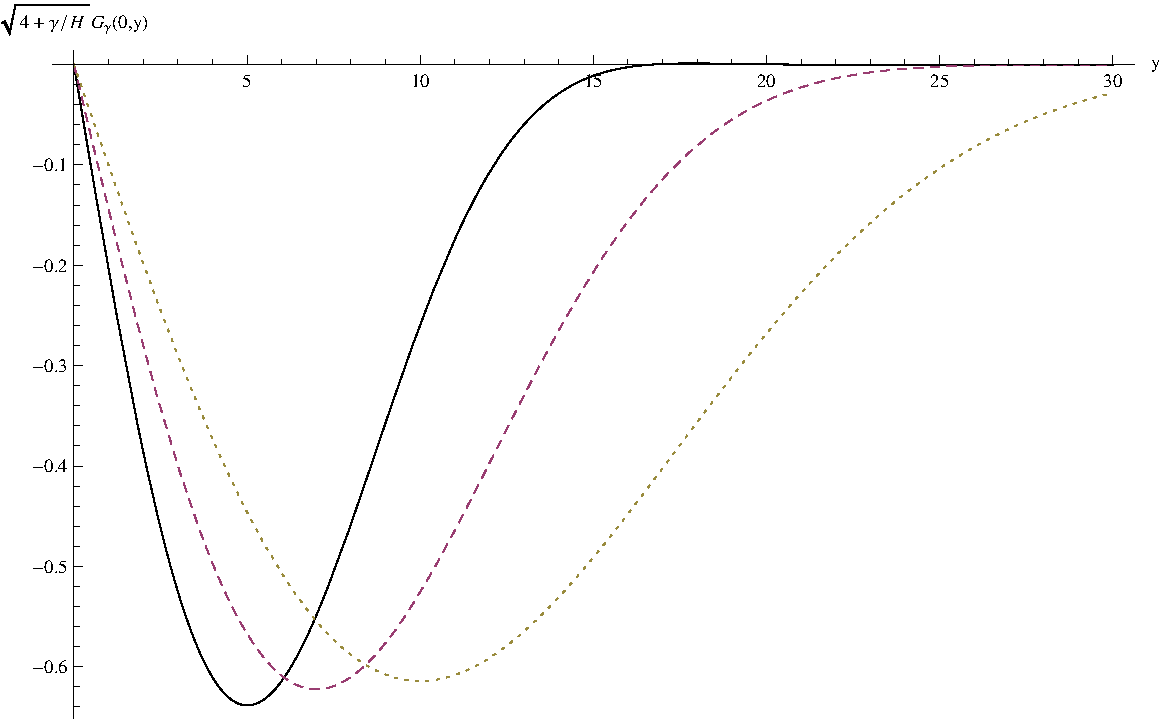
\includegraphics[width=8.5cm]{Greengamma}
\caption{$\gamma$の異なる3つの値に対するGreen関数$G_{\gamma}(0,y)=y^2 g_{\gamma}(0,y)$。$4+\gamma/H=5^2$（黒実線）、$4+\gamma/H=7^2$（破線）、$4+\gamma/H=10^2$（点線）に対し、$G_{\gamma}$の最初のピークはそれぞれ$y=5,\,7,$および$10$付近にあり、ピークの位置が$\sqrt{4+\gamma/H}$であることを裏づけている。}\label{GreGamma}
\end{figure}

\begin{figure}[h]
\centering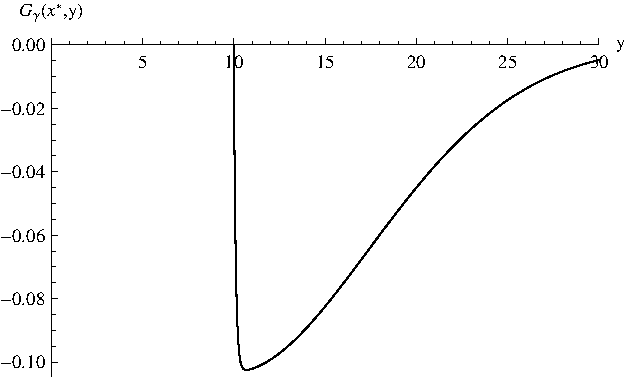
\includegraphics[width=.48\linewidth]{Greengammasqrt}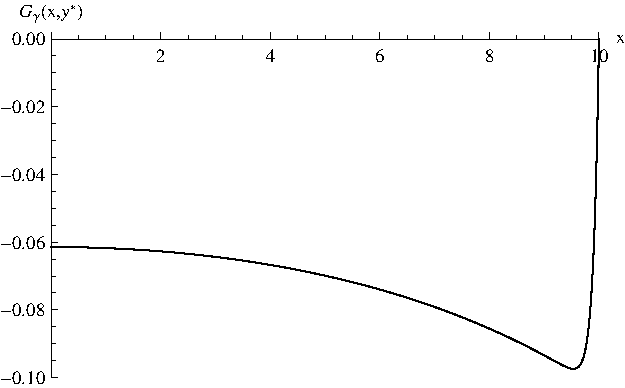
\includegraphics[width=.48\linewidth]{Greengammasqrtx}
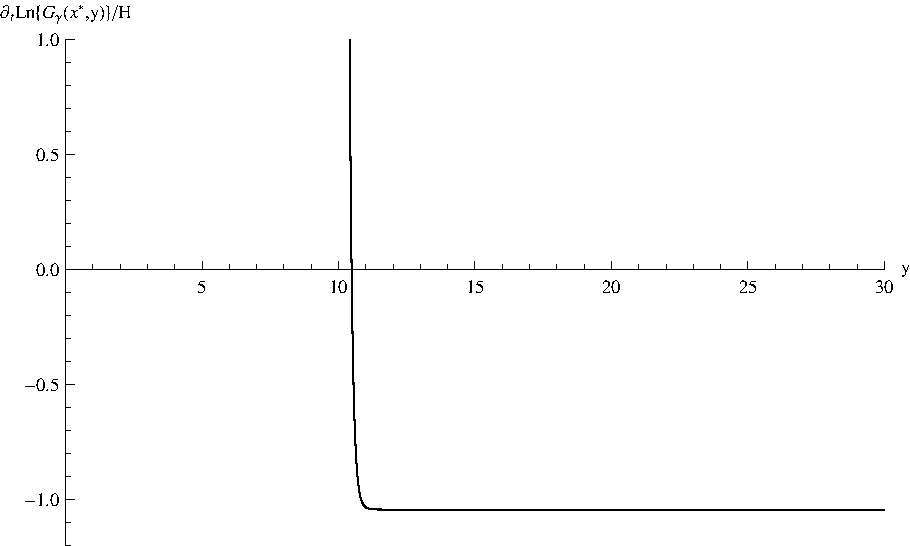
\includegraphics[width=.48\linewidth]{DotGreengammasqrt}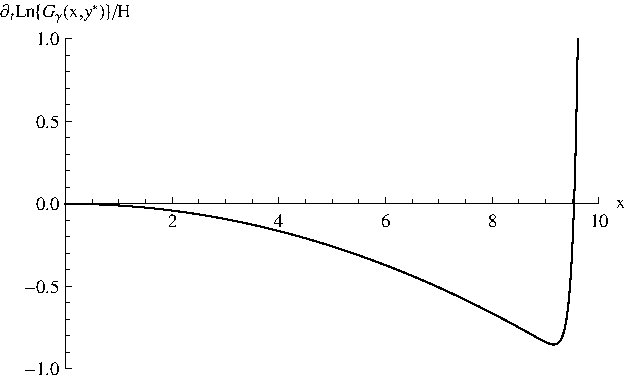
\includegraphics[width=.48\linewidth]{DotGreengammasqrtx}
\caption{Green関数$G_{\gamma}(x,y)$（上段）と、Hubble時間を単位としたその時間微分$\partial_tG_{\gamma}(x,y)/H=-x\partial_xG_{\gamma}(x,y)$（下段）。左列は$x^\star=\sqrt{4+\gamma/H}$を固定した$y>x^\star$の関数、右列は$y^\star=\sqrt{4+\gamma/H}$を固定した$x<y^\star$の関数として示す。すべての図は$x^\star=y^\star=10$に対応する。}\label{GreGamma2}
\end{figure}

ある特定の$\gamma$の値について、図~\ref{GreGamma2}にGreen関数$G_{\gamma}(x,y)$と、Hubble時間を単位としたその時間微分$\partial_tG_{\gamma}(x,y)/H=-x\partial_xG_{\gamma}(x,y)$を示した。$x=\sqrt{4+\gamma/H}$を固定して$y>x$の関数として描いたものと、$y=\sqrt{4+\gamma/H}$を固定して$x<y$の関数として描いたものを示している。$g_{\gamma}$の積分の大きさを見積もるには、
\be
\int_x^{+\infty} dy\, G_{\gamma}(x,y)=-1.
\ee
に注意すると便利である。$\gamma$が大きい場合、$y^2$の各因子を$\gamma$と数え、$G_{\gamma}$ごとに$\gamma^{-1/2}$（すなわち$g_{\gamma}$ごとに$\gamma^{-3/2}$）を、積分ごとに$\gamma^{1/2}$を掛け、$\gamma/H$を用いて単位を整えれば、$f_{\rm NL}^{\rm eq}$の大まかな見積もりが得られる。$G_{\gamma}$にHubble時間を単位とする時間微分があっても、$f_{\rm NL}^{\rm eq}$を大幅には増加させないことに注意されたい（図~\ref{GreGamma2}を参照）。一方、Hubble長を単位とする空間微分が追加されると、その寄与は$f_{\rm NL}^{\rm eq}$をおよそ$\gamma/c_s^2$倍に増加させる（$k^2/(a^2H^2)=y^2/c_s^2$であるため）。

%---------------------------------------------------------------------------

\sectionlink{混合}\label{mixing}

$\pi$の最低次における摩擦の効果を調べるために、本論文では一般的な型の演算子、すなわち$\calo\pi$の研究に集中した。ここで$\calo$には、原理的には（部分積分の後で）一連の寄与が含まれている。しかし、高次の効果を加える際には、それぞれを個別に扱った。その理由は、すべての項が同じ型の非線形性を生成するわけではないこと、そしてもちろん簡単のためでもあった。しかし一般には、複数の演算子が同時に存在する。ここでは、複数の型のADOFを同時に含めた結果として、どのような効果が現れうるかについていくつか述べる。

\subsectionlink{スカラー}\label{mixingscalars}

スカラー演算子$\calo_A$、$A=1,\ldots N$から始めよう。一般に、自己相関関数によって与えられる応答と雑音の寄与に加えて、交差相関（例えば$\langle\delta\calo^S_A\delta\calo^S_B\rangle$）による寄与も存在する。より正確には、次の形の相互作用項を考えている：
\be S_{int}=-\int d^4x a^3(t) \calo_A F^A, \ee
ここで$F^B$は、$\calo$に対応するADOFの動力学をわずかに乱す外力とみなし、繰り返された添字については和をとる。したがって、外力の印加による$\calo_A$の線形応答は
\be \delta\calo_A^R=-\int d^4x' a^3(t') G_{AB}^\calo(x,x') F^B(x'),\label{deltaO}\ee
と書ける。ここで、
\be G_{AB}^\calo(x,x')=i \theta(t-t')\langle[\delta\calo_A(x), \delta\calo_B(x')]\rangle.\ee
である。さらにADOFの揺らぎがあり、これは確率的な源$\delta\calo^S_A(x)$の2点関数によって特徴づけられる：
\be N_{AB}^\calo(x,x')= \langle\delta\calo^S_A(x)\delta\calo^S_B(x') \rangle.\ee

第~\ref{localapp}節で述べた局所近似が適用できる場合に注目すると、
\beq
\label{respoLoc}
 \delta\calo_A^R(t,{\bf k})\simeq \mu_{AB}(t) F^B(t,{\bf k})+\Gamma_{AB}(t)\frac{1}{a^{3/2}} \partial_{t}(a^{3/2}(t) F^B(t, {\bf k})),
\eeq
\beq \langle\delta{{\calo}}_A^S(t,{\bf k}_1)\delta{{\calo}}^S_B(t,{\bf k}_2)\rangle=(2\pi)^3\delta^{(3)}({\bf k}_1+{\bf k}_2)
{N}_{AB}^{\calo}(t,t'),\eeq
と書ける。ただし、
\be  {N}_{AB}^\calo(t,t')\simeq~ \nu_{AB}(t) \frac{ \delta(t-t')}{a^{3}(t)},\ee
であり、$\mu_{AB}(t),\,\Gamma_{AB}(t)$と$\nu_{AB}(t)$は近似的に時間に依存しない。

\subsectionlink{\texorpdfstring{$ f(t)\calo_1$と$\calo_2 g^{00}$}{f(t)O₁とO₂g⁰⁰}}

議論を完備させるために、前述の局所近似の仮定のもとで、$\calo_1$と$\calo_2$の混合による効果を調べよう。この混合を無視すると、相互作用$f_1\calo_1$は$\pi$の運動方程式に$\gamma\dot{\pi}$という項を与える（第\ref{ftcalo}節を参照）。一方、両演算子のGreen関数が$\omega\rightarrow 0$で${\rm Im}\,G(\omega)\propto\omega$を満たすと仮定すると、$\calo_2 g^{00}$は高階微分の寄与を生じる（第\ref{localo2}節を参照）。したがって、一次では$f_1\calo_1$の項が$f_2\delta g^{00}\calo_2$より支配的な場合を考えるのが妥当である。これにより、$\calo_2$によって導入される補正の最低次では、相互作用$\delta g^{00}\calo_2$単独からの寄与を無視でき、その効果が$\calo_1$との混合のみを通じて現れる状況に注目できる。例えば、$\calo_1=\calo_2$かつ$f_2 H\ll\dot{f_1}$であればこの場合に該当する。したがって実際には$f_2$の最低次で計算できる。さらに簡単のため、ここでは線形応答近似を用いて得られる寄与だけに注目する。ただし、第\ref{localo2}節で見たように、$ f_1\calo_1$から得られる非線形応答の寄与が、この種の模型で最大の非Gaussian性を生成する可能性がある\footnote{第\ref{ftcalo}節の解析から、相互作用$f_1\calo_1$だけが存在する場合、線形応答近似の範囲で得られる非Gaussian性は無視できるほど小さいことに注意されたい。}。

混合による応答項には2つの型がある。一方は$f_1(t)$（$\calo_1$に結合する力）が$\delta\calo_2$に及ぼす影響によるものであり、もう一方は$f_2\delta g^{00}$が$\delta\calo_1$に及ぼす影響によるものである。局所近似を用いると、これらは
\begin{subequations}
\begin{align}
\delta\calo_1^{R_{\rm mix}}&\simeq~ -f_2\tilde{\mu}_{12}\lp 2\dot{\pi}+\dot{\pi}^2-\frac{\partial_i\pi\partial_i\pi}{a^2}\rp\nonumber\\
&-f_2\Gamma_{12}\lp2\ddot{\pi}+2\dot{\pi}\ddot{\pi}-2\frac{\partial_i\pi\partial_i\dot{\pi}}{a^2}+2H\frac{\partial_i\pi\partial_i\pi}{a^2}\rp,\\
\delta\calo_2^{R_{\rm mix}}&\simeq~ \tilde\mu_{21}\lp\dot{f_1}\pi+\ddot{f_1}\frac{\pi^2}{2}\rp+\Gamma_{21}\lp\dot{f_1} \dot{\pi}+\ddot{f_1}\dot{\pi}\pi\rp,
\end{align}
\end{subequations}
と書ける。ここで$\tilde{\mu}_{AB}={\mu}_{AB}+3/2H\Gamma_{AB}$であり、本文で述べたような創発的シフト対称性が存在すると仮定した。

$f_2$の一次までで、$\pi_1$の方程式は
\be
\ddot{\pi}_1+(3H+\tilde{\gamma})\dot{\pi}_1+\tilde{c}_s^2\frac{\nabla^2}{a^2}\pi_1=-\tilde{N}_c^{-1}
\left(\dot{f_1}\delta\calo_1^S-2f_2\frac{\partial_t(a^3\delta\calo_2^S)}{a^3}\right),
\ee
となる。ここで$\tilde{N}_c=N_c+2f_2\dot{f_1}(\Gamma_{21}-\Gamma_{12}))$、$\tilde{c}_s^2={c}_s^2-2f_2\tilde{N}_c^{-1}\dot{f_1}c_s^2(\Gamma_{21}-\Gamma_{12})$、$\tilde{\gamma}= \tilde{N}_c^{-1}\left(\dot{f_1}^2\Gamma_{11}+2f_2\dot{f_1}(3H\Gamma_{12}-\tilde{\mu}_{12})\right)$である。$\tilde{c}_s^2\tilde{N}_c=c_s^2N_c $が成り立つことに注意されたい（$f_2$の一次までで計算していることを思い出そう）。記法を簡単にするため、以下ではチルダを省略する。上の方程式の特解は
\begin{eqnarray}
\pi_1(k,\eta)&=&\frac{\dot{f_1} k c_s}{N_cH^2}\int^{\eta}_{\eta_0} d\eta'g_{\gamma}(kc_s|\eta|,kc_s|\eta'|)\delta\calo_1^S({\bf k},\eta')\nonumber\\
&+&\frac{2 f_2 k c_s}{N_cH^2}\int^{\eta}_{\eta_0} d\eta'g_{\gamma}(kc_s|\eta|,kc_s|\eta'|)\frac{\partial_t \lp a^3(\eta')\delta\calo_2^S({\bf k},\eta')\rp}{a^3(\eta')},
\end{eqnarray}
であり、得られるパワースペクトルは
\be
P_{\zeta}=P_{\zeta}^{f_2=0}\lp 1+6\frac{H f_2\nu_{12}} {\dot{f_1}\nu_{11}}\rp
\ee
と書ける。$P_{\zeta}^{f_2=0}$は$f_2=0$で得られるものであり、式~(\ref{pow1gamma})で$\nu_\calo=\nu_{11}\dot{f_1}^2$としたものである。$\pi$に対する源は
\begin{eqnarray}
J&=&N_c^{-1}\dot{f_1}(2f_2H\Gamma_{12}-f_2\tilde{\mu}_{12}) \frac{\partial_i\pi\partial_i{\pi}}{a^2}-2N_c^{-1} f_2\dot{f_1}(\Gamma_{12}-\Gamma_{21})\frac{\partial_i\pi\partial_i\dot{\pi}}{a^2}\nonumber\\
&+&2f_2N_c^{-1}\dot{f_1}\Gamma_{21} \dot{\pi}\frac{\nabla^2\pi}{a^2}+f_2N_c^{-1}\dot{f_1}(\tilde{\mu}_{12}-6H\Gamma_{21})\dot{\pi}^2+2f_2N_c^{-1}\dot{f_1}(\Gamma_{12}-2\Gamma_{21})\dot{\pi}\ddot{\pi}\nonumber\\
&-&\dot{f_1}\delta\calo_1^S-2f_2\frac{\partial_t\lp a^3\delta\calo_2^S\rp}{a^3}-2f_2\frac{\partial_t\lp a^3\dot{\pi}\delta\calo_2^S\rp}{a^3}+2f_2N_c^{-1}\frac{\partial_i\lp\delta\calo_2^S\partial_i\pi\rp}{a^2}.\label{mixsource}
\end{eqnarray}
となる。$\calo_1=\calo_2$なら第2項は消えることに注意されたい。\\

第\ref{nongaus}節の計算からわかったように、非Gaussian性を生成するうえでは、空間微分をもつ非線形項の寄与が、時間微分だけをもつ項の寄与よりも重要となる。そこで簡単のため、主要な項に含まれると予想される最初と最後の項だけを調べよう。最初の源の項についての計算は、第\ref{Nolocalo2}節で式~(\ref{pieqnl})の右辺第1項に対してすでに行った計算とまったく同じである。実際、これは
\be J_k^1=-s_1\gamma\frac{\partial_i\pi\partial_i{\pi}}{a^2},\ee
と書ける。ただし、
\be
s_1=-\frac{2f_2 H}{\dot{f_1}}\frac{\Gamma_{12}}{\Gamma_{11}} +\frac{f_2\tilde{\mu}_{12}} {\dot{f_1}\Gamma_{11}}, \ee
である。簡単のため$\gamma_{AB}\sim H \mu_{AB}$とすると、$f_2$についての線形展開と整合するように$s_1\ll 1$となる。式~(\ref{fnlgoonoloc})から
\beq f_{\rm NL}^{\rm eq}\simeq\frac{s_1\gamma}{2H c_s^2},\eeq
を得る。$c_s\lesssim 1$であり、近似が有効な範囲、すなわち$s_1 \ll 1$であっても、$\gamma\gg H$であればこれは依然として大きくなりうる。\\

同様に、源の最後の項については
\begin{eqnarray}
f_{\rm NL}^{\rm eq}&=&-\frac{10}{3}\frac{s_2}{c_s^2}\frac{2^{-8\gamma/H}\pi^2 {\Gamma\left(\frac{2\gamma}{H}+4\right)}^2}{\lp\frac{\gamma}{H}+1\rp^6{\Gamma\lp\frac{\gamma+H}{2 H}\rp}^8}
 \int_{0}^{+\infty} dy' {y'}^6 (g_{\gamma}(0, y'))^2\nonumber\\&\times&\int_{y'}^{+\infty} dz z^4  g_{\gamma}( y',z)g_{\gamma}(0, z),\label{fnlmix2n}
\end{eqnarray}
を得る。ここで$s_2=\frac{f_2H}{\dot{f_1}}\frac{\nu_{12}}{\nu_{11}}\ll 1$であり、再び簡単のため、すべての質量スケールは同程度とした。数値計算を行うと、$\gamma/H\gg 1$の領域では$f_{\rm NL}$を
\beq
f_{\rm NL}^{\rm eq}\simeq- 3\frac{\gamma}{H} \frac{s_2}{ c_s^2},
\eeq
によってよく近似でき、前の場合と同様の結果となる。

\subsectionlink{ベクトルとテンソル}\label{vectens}

最後に、第\ref{vectors}節および第\ref{tensors}節で論じたように、追加できる一群のベクトルおよびテンソル相互作用項がある。これらは
\begin{eqnarray}\label{family}
S^{\calo}&=&-\int d^4 x \sqrt{-g}\,\left(f_1(t)\calo^{0}_1+f_2(t)\calo^{00}_2+f_3(t)\calo^{000}_3+\ldots\right) \\
&-&\delta g^{00}\left(s_1(t)\calo^{0}_1+s_2(t)\calo^{00}_2+s_3(t)\calo^{000}_3+\ldots\right)+\ldots\nonumber
\end{eqnarray}
と書ける。

議論と記法を簡単にするため、ここでは、一般にその時間依存性がスローロールで抑制される因子$f_i(t)$と$s_i(t)$を省略しよう。\\

$\pi$を導入すると、これらの項は
\begin{subequations}\begin{align}
\calo^{0}_1&=\calo^{\mu}_1\partial_{\mu}(\tilde{t}+\pi)=\calo^{0}_1+\calo^{\mu}_1\partial_{\mu}\pi\\
\calo^{00}_2&=\calo^{\mu\nu}_2\partial_{\mu}(\tilde{t}+\pi)\partial_{\nu}(\tilde{t}+\pi)\\&=\calo^{00}_2+2\calo^{0\mu}_2\partial_{\mu}\pi+\calo^{\mu\nu}_2\partial_{\mu}\pi\partial_{\nu}\pi\nonumber\\
\calo^{000}_3&=\calo^{\mu\nu\rho}_3\partial_{\mu}(\tilde{t}+\pi)\partial_{\nu}(\tilde{t}+\pi)\partial_{\rho}(\tilde{t}+\pi)\\&=\calo^{000}_3+3\calo^{00\mu}_3\partial_{\mu}\pi+3\calo^{0\mu\nu}_3\partial_{\mu}\pi\partial_{\nu}\pi+\calo^{\mu\nu\rho}_3\partial_{\mu}\pi\partial_{\nu}\pi\partial_{\rho}\pi,\nonumber
\end{align}
\end{subequations}
などとなる。これらをすべて足し合わせると、
\be\label{suma}
\calo^{0}_1+\calo^{00}_2+\calo^{00}_3+\ldots=\tilde{\calo}+\tilde{\calo}^{\mu}\partial_{\mu}\pi+\tilde{\calo}^{\mu\nu}\partial_{\mu}\pi\partial_{\nu}\pi+\tilde{\calo}^{\mu\nu\rho}\partial_{\mu}\pi\partial_{\nu}\pi\partial_{\rho}\pi \ldots,
\ee
を得る。$\tilde \calo^{\mu\ldots\nu}$は、もとのテンソル演算子の何らかの組み合わせから構成される。式~(\ref{family})の第2行も同様に並べ替えることができる。\\

例として、式~(\ref{suma})の最初の$\pi$に依存する項を生成する$\calo^0 \equiv \calo_\mu g^{\mu0}$を考えよう。式を見ればわかるように、$\pi$の一次では、この演算子の解析は、本論文を通して調べてきたスカラー演算子の解析へと帰着できる。実際、部分積分すると、
\beq \label{oeff} \int d^4x \sqrt{-g} \calo^\mu \partial_\mu \pi \to \int d^4x \left(\partial_\mu \sqrt{-g} \calo^\mu\right)\pi \equiv \int d^4x \sqrt{-g} \tilde\calo \pi,
\eeq
を得る。ここで$\tilde\calo= \frac{1}{\sqrt{-g}}\partial_{\mu}(\sqrt{-g}{\calo}^{\mu})$は有効スカラー演算子である。この相互作用は構成のしかたからシフト対称性を満たす。さらに、第\ref{localapp}節の仮定を満たすならば、$\gamma \gg H$に対して大きな摩擦項を誘起しうるが、作用中には$O(\pi^2)$の項が生じない。素朴には、この場合には摩擦と非Gaussian性に関係がないように思えるかもしれない。しかし、本論文全体を通じて強調したように、非線形応答は非線形結合を誘起する。これらは実際に大きいと予想され、$f_{\rm NL} \simeq\gamma/c_s^2H$を与える。

%-------------------------------------------

\sectionlink{\texorpdfstring{$\gamma\dot\pi$型の散逸を伴う$\calo\delta g^{00}$模型}{γ π̇型の散逸を伴うO δg⁰⁰模型}}\label{mag00}

この付録では、$\gamma\dot\pi$型の散逸を伴う$\tilde\calo g^{00}$型の結合の例を議論する。第\ref{storyo}節で論じたように、これには特殊な解析構造が必要であり、特に、間もなく定める周波数域$\mu_\calo < \omega < \Gamma_\calo$において（式(\ref{tildG})を参照）、
\beq
{\rm Im} \tilde G_{\rm ret}^\calo (\omega) \sim 1/\omega,
\eeq
が必要となる。ここでは、インフラトンを、$\pi$とは直接結合しない第2の（隠れた）セクターによって強い散逸的動力学を与えられるスカラー場に結合させる、一つの可能な模型を導入する。この設定については別の機会にさらに詳しく調べる予定である。（以後はチルダを省略し、また多数の$\gamma$が現れるため、$\pi$の散逸係数を$\gamma_\pi$と表す。）\\

基本的な考え方は文献\cite{eft1}のインフレーションのEFTを用いることである。ただし、文献\cite{dan2}の模型と同じ考えに基づき、$\sigma \delta g^{00}$という項を通じて$\pi$をスカラー場$\sigma$に結合させ、質量の単位をもつ$\rho$を係数とする$\rho \sigma\dot\pi$結合を生成する\cite{dan2}。その動力学を
\beq
\calL_\sigma = \frac{1}{2}(\partial_\mu \sigma)^2 - \frac{1}{2} \mu^2 \sigma^2 + \sigma J_\Psi,
\eeq
と書く。ここで$J_\Psi$は、$\sigma$と、まとめて$\Psi$と表される散逸セクターとの相互作用を表す。このセクターは$\pi$とは直接結合しない。\footnote{原理的には$\Psi$は重力相互作用を通じてインフラトンと相互作用しうるが、それらは劣勢の寄与である。}本質的には、これは$\pi$が混合項を介して散逸する2段階の模型である。文献\cite{multieft}の枠組みでも記述できるが、ここではさらに、$\sigma$に結合して（強い）散逸を誘起するセクターが存在する。（例えば、$\Psi$系をある温度$T_\Psi$の熱平衡状態に置いてもよい。）\\

ここで$\sigma$の遅延Green関数を計算すると、次式を得る（図\ref{odot}を参照）：
\beq
\rho^2 G^\sigma_{\rm ret}(\omega,{\bf k}) = \frac{\rho^2}{\omega^2-{\bf k}^2 - \mu^2 + \Gamma_\Psi(\omega)},
\eeq
ここで$\Gamma_\Psi$は、$\sigma J_\Psi $結合による$\langle[ J_\psi, J_\psi] \rangle$相関関数からの自己エネルギー寄与である（後述）。この自己エネルギーの虚部を
\beq
\label{imsigm}
{\rm Im}\, \Gamma_\Psi(\omega) \simeq \gamma_\Psi \frac{\omega}{\omega+\Lambda_\psi},
\eeq
と近似できると仮定しよう。これはより標準的な振る舞い（式(\ref{drude})のDrude模型に類似）であり、$\omega < \Lambda_\psi$では$\omega$に対して線形に振る舞う。付録\ref{appB}を参照されたい。上半平面における$\Gamma_\Psi$の解析性を用いると、（Kramers-Kronig関係を通じて）$\omega \lesssim \Lambda_\Psi$に対し
\beq
\label{resigm}
{\rm Re}\,\Gamma_\Psi(\omega) \simeq \gamma_\Psi \Lambda_\Psi \left(\frac{\Lambda_\Psi^2}{\omega^2+\Lambda_\Psi^2}\right) \simeq \gamma_\Psi \Lambda_\Psi,
\eeq
も得られる。したがって、
\beq
\label{imGs}
\rho^2 {\rm Im}\, G^\sigma_{\rm ret}(\omega,{\bf k}) \simeq  \frac{\gamma_\Psi \rho^2 \omega}{\left[\omega^2-{\bf k}^2 - \mu^2 + \gamma_\Psi \Lambda_\Psi \right]^2 + \gamma_\Psi^2\omega^2}.
\eeq

\begin{figure}[h!]
\centering
    \centering
    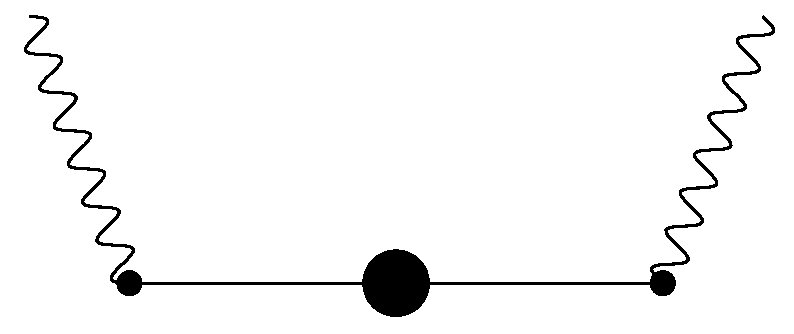
\includegraphics[width=6.5cm]{odotfig_cropped}
\caption{波線は$\pi$に対応し、黒い相互作用点は$\sigma\dot\pi$結合の挿入である。大きな黒丸は、$\sigma J_\Psi $結合から生じる$\langle [J_\psi, J_\psi]\rangle$相関関数のGreen関数を表す。}
\label{odot}
\end{figure}

ここで求めたいのは、運動方程式に$\gamma_\pi \dot\pi_k$が得られる領域、言い換えると、式(\ref{tildG})のスケーリングが式(\ref{imGs})で実現する領域である。これは実際、
\beq
\label{mutuned2}
\left[\omega^2-{\bf k}^2 - \mu^2 + \gamma_\Psi \Lambda_\Psi \right]^2 \ll \gamma_\Psi^2\omega^2.
\eeq
の場合に実現する。

$\omega\lesssim \Lambda_\Psi$という制約を考えると、素朴にはこれを実現するのは難しそうに見える。しかし、大きな寄与を打ち消すように$\mu$を設定することは常に可能である。例えば、\footnote{（保護されていない）スカラー場を扱う際に、ある程度の微調整が必要になることは驚くべきことではない。一つの可能性は、$\sigma$を擬Goldstoneボソンとみなすこと、あるいは対称性の破れのスケールをHubbleスケール付近とした超対称な版を導入することである。（その意味で、これは文献\cite{multieft}の超対称多場インフレーションのEFTに似ている。文献\cite{dan2new}も参照。）この問題は今後の課題として残す。}
\beq
\label{mutuned}
\gamma_\Psi \Lambda_\Psi - \mu^2 \simeq H^2.
\eeq
と調整すればよい。さらに$\omega_\star, k_\star \ll \gamma_\Psi$も仮定する（これは自己無撞着であることを後に示す）。すると、採用した仮定のもとで、$H \lesssim  \omega, |{\bf k}| \lesssim \gamma_\Psi (\lesssim \Lambda_\Psi)$に対し
\beq
\label{imGs2}
\rho^2 {\rm Im}\, G^\sigma_{\rm ret}(\omega) \simeq  \frac{\gamma_\Psi \rho^2}{\gamma_\Psi^2}\frac{1}{\omega},
\eeq
を得る。したがって、
\beq
\gamma_\pi \sim \frac{\rho^2}{\gamma_\Psi},
\eeq
であり、$\rho \sim \gamma_\Psi$の場合には$\gamma_\pi \sim \gamma_\Psi$となる。本論文で示したように、$\gamma_\pi\dot\pi$という散逸項がある場合には$k_\star \simeq \sqrt{\gamma_\pi H}$となるため、$\gamma_\pi \gg H$であれば式(\ref{imGs2})を導いた条件は満たされる。\\

パワースペクトルと非Gaussian性を計算するためには、雑音部分も必要である。これもまた、$\sigma$を介した$\pi$と$J_\Psi$の（間接的な）結合から従う。このことは、運動方程式を明示的に書けば示せる（簡単のためHubble膨張を無視する）：
\bea
\label{ddpis}\ddot\pi_k + k_{\rm ph}^2\pi_k &=& -\rho\dot\sigma_k, \\
\label{ddsig}\ddot\sigma_k + (k_{\rm ph}^2+\mu^2)\sigma_k &=& J_\Psi + \rho\dot\pi_k.
\eea

上で論じたように、関心のある領域では（$J_\Psi$を特定の演算子~$\delta\calo$とみなして）、
\beq
J_\Psi =  J^S_\Psi + \int G^\Psi_{\rm ret} \sigma \simeq J^S_\Psi +\gamma_\Psi\Lambda_\Psi\sigma - \gamma_\Psi\dot\sigma,
\eeq
と書ける。ここでは式(\ref{imsigm})および(\ref{resigm})を用い、先ほどと同様に確率的な源の項$J^S_\Psi$を加えた。したがって、式(\ref{mutuned2})に従って$\mu$を選ぶと、
\beq
 \gamma_\Psi\dot\sigma_k \simeq \rho\dot \pi_k - J^S_\Psi,
\eeq
となり、これを式(\ref{ddpis})に代入すると最終的に
\beq
\ddot\pi_k + k_{\rm ph}^2\pi_k +\gamma_\pi \dot\pi_k = J^S_\pi,
\eeq
を得る。ただし$J^S_\pi =\left(\rho/\gamma_\Psi\right) J^S_\psi$である。このように式(\ref{eom1})と同じ形の方程式が残り、本論文を通じて行った計算が適用できる。特に、第~\ref{Nolocalo2}節と同様に$f_{\rm NL} \simeq \gamma_\pi/(c_s^2 H)$程度の非Gaussian性を得る。\\

$\sigma$をゲージ結合$g A^\mu \partial_\mu \pi$に置き換えることで、${\calo}_\mu g^{\mu0}$型の演算子についても同様の模型を構成できることに注意されたい。その場合、$J_\Psi$は通常の電磁電流と同様の役割を果たす（付録\ref{appB}を参照）。

\sectionlink{局所的なトラップ型インフレーションの整合性}\label{consistency}

ここでは、近似の妥当性を保証する基本的な制約をいくつかまとめる。背景方程式については、
\be\label{c5c6} |\ddot{\phi}|\ll 3H|\dot{\phi}|\ll V'(\phi),\ee
が必要であり、このとき等速度の解
 \be\label{E1} \dot{\phi}\simeq~ -\frac{(\Gamma_\chi|\Delta|(2\pi)^3 V')^{2/5}}{g}.\ee
が得られる。さらに、エネルギー密度はポテンシャルエネルギーに支配されると仮定する：
\be\label{EnDens} 3M_p^2 H^2=\frac{\dot{\phi}^2}{2}+V(\phi)+\sum_i M_{\chi_i} n_{\chi_i}\simeq V(\phi).\ee
一般化されたスローロールパラメータ$\epsilon=-\dot{H}/H^2$は、
\be\epsilon=\frac{3(\dot{\phi}^2+\sum_i M_{\chi_i} n_{\chi_i})}{2 V(\phi)}.\ee
で与えられる。したがって、$\epsilon\ll 1$から
\begin{subequations}\begin{align}
&\dot{\phi}^2\ll V(\phi),\label{c7}\\
&\sum_i M_{\chi_i} n_{\chi_i}\ll V(\phi),\label{c8}
\end{align}\end{subequations}
が従う。これらは式(\ref{EnDens})の近似に必要な条件である。式(\ref{c8})の左辺を見積もるため、上と同様に和を積分に置き換えると、
\be
\sum_i M_{\chi_i} n_{\chi_i}\simeq~\frac{g^{5/2}|\dot{\phi}|^{7/2}}
{\Gamma_{\chi}^2|\Delta|(2\pi)^3}\ll V(\phi).
\ee
を得る。すべての条件をまとめると、式(\ref{c1})、(\ref{c2n})、(\ref{c3c4})、(\ref{c5c6})、(\ref{c7})、(\ref{c8})に加えて、$k_{\rm ph} \ll \kappa$、$k_{\rm ph}\Delta \ll |\dot \phi|$、さらに$\Gamma_\chi\gg H$という条件がある。また、e-fold数についても
\be \label{efolds}N_e=\int \frac{H}{\dot{\phi}}d\phi=\frac{5 g m \phi ^2}{16 2^{7/10} \sqrt{3} \pi ^{6/5} \left(m^2 \Gamma_\chi  \Delta  \phi \right)^{2/5}},\ee
を得る。ここでは$\phi\equiv\phi_I \gg\phi_E$を用いており、$\phi_I$（$\phi_E$）はインフレーションの開始時（終了時）におけるインフラトン場の値である。

\begin{figure}[h!]
\centering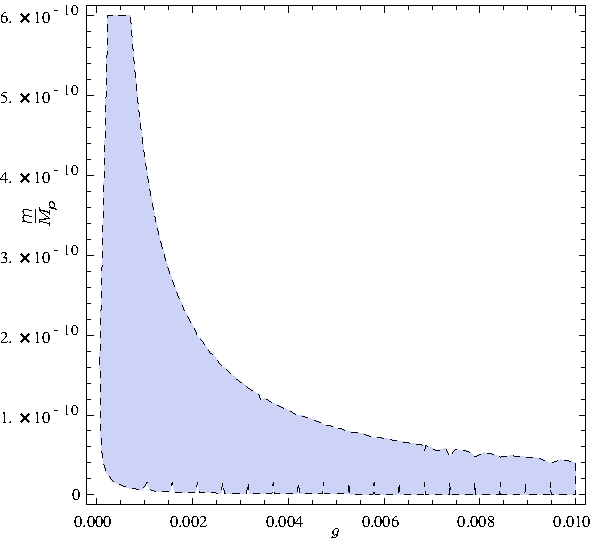
\includegraphics[width=.48\linewidth]{TrapdecayCuadgama100HFin}
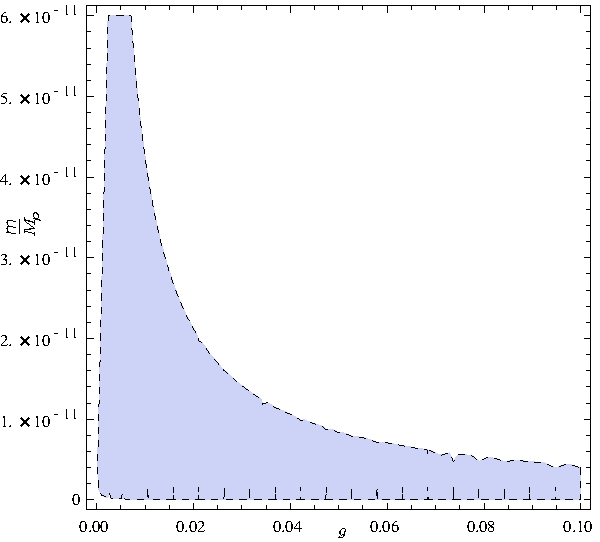
\includegraphics[width=.48\linewidth]{TrapdecayCuadgama1000HFin}
\caption{整合性によって許される自由パラメータ（$m$と$g$）の領域（$``\ll"$を$``<"$に置き換えた）。横軸は$g$、縦軸は$m/M_p$を表す。左：$\Gamma_\chi=100 H$（場合I）、右：$\Gamma_\chi=1000 H$（場合II）。}
\label{RR}
\end{figure}

次に、代表的な例である
\be V(\phi)=\frac{m^2}{2}\phi^2.\ee
について、これらの制約を調べる。

この模型には、$m,\,\Delta,\,\Gamma_\chi,\,g$と、インフラトン場の初期値$\phi_I$の5つのパラメータがある。パラメータ空間を縮小するため、$N_e=60$および
\beq
P_{\zeta}\simeq\lp\frac{H}{\dot{\phi}}\rp^2P_{\delta\phi}\simeq \frac{10^{-9}}{k^3},
\eeq
を課す。これより、次の条件を得る（式(\ref{zeta2nu})を参照し、$N_c \simeq \dot\phi^2$を用いる）：
\beq\label{E2}
\lp\frac{H}{\dot{\phi}}\rp^2 \frac{g^2\nu_{\chi}}{4}\lp\frac{\pi H}{\gamma}\rp^{1/2}\simeq 10^{-9}.
\eeq
すると、
\begin{equation}\phi \simeq \frac{16 2^{3/16} 3^{15/16} \pi ^{3/4} \sqrt[4]{\Gamma_\chi  |\Delta| }}{\sqrt[8]{g^5 m}} M_p,~~
|\Delta|\simeq\frac{1179648\times 10^{34} \sqrt[4]{6} \pi ^{11} g^{13/2} m^{9/2} M_p}{\Gamma_\chi }
\end{equation}
となる。簡単のため、$\Gamma_\chi=100 H$（場合I）と$\Gamma_\chi=1000 H$（場合II）の2つの場合を調べる。図~\ref{RR}には、すべての条件を満たすパラメータ$m$と$g$の2次元領域を示した（$``\ll"$を$``<"$に置き換えた）。横軸は$g$、縦軸は$m/M_p$を表し、場合Iが左のグラフ、場合IIが右のグラフに対応する。例として$\Gamma_\chi=100 H$、$m=10^{-11}M_p$、$g= 10^{-2}$とすると、$H\simeq 1.3\times 10^{-11} M_p$、$\gamma/H\simeq  135$、$\phi\simeq 3.3 M_p$、$\delta t_c \simeq 1.98 \times 10^{-4} H^{-1}$、$|\Delta|\simeq 1.29\times 10^{-8}M_p$、$\epsilon\simeq 1/32$を得る。また、$\Gamma_\chi=1000 H$、$m=5\times 10^{-13}M_p$、$g= 10^{-1} $に対しては、$H\simeq 3.34\times 10^{-13} M_p$、$\gamma/H\simeq 539$、$\phi\simeq 1.63 M_p$、$\delta t_c \simeq 1.4\times 10^{-5} H^{-1}$、$|\Delta|\simeq 2.27\times 10^{-7} M_p$、$\epsilon\simeq 1/32$を得る。すべての場合に$\gamma/H \ll g|\dot\phi|/H^2$であり、これは局所近似$k_\star\lesssim \kappa$の妥当性を保証する。最後の確認として、理論に追加したスカラー自由度の揺らぎから生じる曲率摂動の大きさを見積もろう。文献\cite{trapped}に従い、この寄与は
\beq
M_p^2\frac{\partial_i^2}{a^2} \delta g_\chi \sim M_\chi \Delta n_\chi,
\eeq
を計算することによって見積もれる。ここでは$M_\chi(\delta t_c) \simeq g |\dot\phi| \delta t_c \simeq \sqrt{g|\dot\phi|}$とする。上式の$\delta g_\chi$は曲率摂動$\zeta_\chi$そのものではないが、それでも誘起される曲率の大きさの目安を与える。比較のため、この式を$k/a \simeq H$で評価すると、
\beq
\langle\delta g_\chi\delta g_\chi\rangle \simeq \frac{(g|\dot\phi|)^{5/2}N_{\rm hits}}{HM_p^4}.
\eeq
を得る。一方、第\ref{power}節の解析から（式(\ref{nunhits})を参照）、
\beq
\langle\zeta_\phi\zeta_\phi\rangle \simeq \sqrt{H/\gamma} \frac{H^2}{\dot\phi^2} \frac{g^2(g|\dot\phi|)^{3/2}N_{\rm hits}}{\Gamma_\chi}.
\eeq
が得られる。したがって、$\dot\phi^2 \sim \epsilon_\phi V$（$\epsilon_\phi < \epsilon$）を用いると、
\beq
 \frac{\langle\delta g_\chi\delta g_\chi\rangle}{\langle\zeta_\phi\zeta_\phi\rangle} \simeq \frac{\Gamma_\chi k_\star}{M_\chi^2} \epsilon_\phi^2 \ll 1,\eeq
となる。これは$\Gamma_\chi\lesssim M_\chi\,, k_\star\lesssim M_\star$かつ$\epsilon_\phi\lesssim 1$であるためである。したがって、これらの曲率摂動は劣勢となる。




